\documentclass[12pt,a4paper]{article}

\usepackage{geometry}
\usepackage[utf8]{inputenc}
\usepackage[T1]{fontenc}
\usepackage{graphicx}
\usepackage{hyperref}
\usepackage[french]{babel}
\usepackage{listings}
\usepackage{color}

\definecolor{green}{rgb}{0,0.6,0}
\definecolor{red}{rgb}{1.0,0.28,0.31}
\definecolor{blue}{rgb}{0.2,0.6,0.8}
\definecolor{orange}{rgb}{1,0.46,0.26}
\definecolor{grey}{rgb}{1,0.8,0.8}
\definecolor{num}{rgb}{0.6,0.2,0.4}
\definecolor{black}{rgb}{0.31,0.31,0.31}
\definecolor{backcolour}{rgb}{0.95,0.95,0.92}
\newcommand{\mylisting}[2][]{%
    \lstinputlisting[caption={\texttt{\detokenize{#2}}},#1]{#2}%
}

\def\code#1{\texttt{#1}}

\lstdefinestyle{customc}{
  language=C,
  showstringspaces=false,
  backgroundcolor=\color{backcolour},
  basicstyle=\footnotesize\ttfamily\color{black},
  keywordstyle=\bfseries\color{orange},
  commentstyle=\itshape\color{red},
  identifierstyle=\color{blue},
  stringstyle=\color{green},
  numbers=left,
  frame=single,
}

\lstset{style=customc,literate=%
    {0}{{{\color{num}0}}}1
    {1}{{{\color{num}1}}}1
    {2}{{{\color{num}2}}}1
    {3}{{{\color{num}3}}}1
    {4}{{{\color{num}4}}}1
    {5}{{{\color{num}5}}}1
    {6}{{{\color{num}6}}}1
    {7}{{{\color{num}7}}}1
    {8}{{{\color{num}8}}}1
    {9}{{{\color{num}9}}}1, 
    morekeywords={@module, @import, @implementation, @class}
    }

\geometry{
  a4paper,
  total={170mm,257mm},
  left=20mm,
  top=20mm,
}

\begin{document}

\title{\Huge{E P I T E C H}\\[2cm]
  \vspace{3pt}\hrule\vspace{6pt}
  Programmation Orientée Objet Avancée \\
  \Large Documentation de conception du projet KOOC
  \vspace{3pt}\hrule\vspace{1.5cm}
}

\author{Alexis Mongin \\
  \and
  Géraldine Heuse\\
  \and
  Christopher Paccard\\
  \and
  Pierre Rousselle\\
  \and
  Benoit de Chezelles\\
  \and
  David Galy\\[12cm]}

\maketitle
\newpage

\begin{NoHyper}
  \tableofcontents
  \newpage
  \section{Introduction \& fonctionnalités}
  Le présent document constitue la documentation de conception d'un compilateur d'un langage orienté objet étendant la grammaire du C, le KOOC (Kind Of Objective C) vers C. Nous détaillerons ici les différentes fonctionnalités du langage. En annexe, nous proposons un exemple de fichier a compiler.
  \subsection{Les modules}
  Un module désigne un ensemble de symboles (variables et fonctions) lui appartenant. Semblable au namespace du C++, il est composé en terme de code d'un bloc de définition \code{@module} contenant ses variables et ses prototypes de fonctions ; et d'un bloc \code{@implementation} contenant cette dernière. Les blocs \code{@implementation} sont situés dans les fichiers .kc et les fichiers contenant les blocs \code{@module} ont pour extension .kh, l'équivalent des headers C. Nous utilisons, dans une unité de compilation, la déclaration \code{@import} afin d'importer les headers KOOC de notre choix
  \subsection{Le polymorphisme ad hoc}
  Les modules peuvent posséder des fonctions avec le même nom, mais des signatures différentes. La signature d'une fonction est l'ensemble des types de ses paramètres ainsi que son type de retour \footnote{Il est intéressant de noter que le type de retour ne fait pas partie des signatures de fonction en C++.}. On implémente ainsi une forme de polymorphisme ad hoc.
  \subsection{Programmation orientée objet}
  Le KOOC est un langage de programmation orienté objet, fournissant a l'utilisateur l'abstraction nécessaire afin de développer selon ce paradigme. Cela se traduit par la présence de types abstraits, possédant des fonctions et des variables membres ; pouvant hériter les uns des autres et possédant des fonctions virtuelles.

  \section{Modules}
  \subsection{Import de module}
  La directive \code{@import} sera remplacée par un \code{\#include} du fichier .h généré par la compilation du fichier .kh concerné. Pour éviter la double inclusion, une macro protectrice sera définie dans chacun des fichiers .h généré. L'import de module, au moment de la compilation, importera aussi les types KOOC tel que les classes, afin de pouvoir reconnaître les déclarations.

\subsection{Compilation des implémentations de module}
  La compilation des blocs \code{@implementation} contenus dans les fichiers .kc se fera simplement en traduisant le nom des symboles kooc vers le nom des symboles C générés.
  \paragraph{Définitions de module\\}
  Les blocs \code{@modules} contenus dans les fichiers .kh seront compilés en calculant d'abord les noms décorés des fonctions dans chaque module présent dans le fichier, puis en copiant leurs prototypes dans le fichier .h de sortie.
Lorsqu'un même module est importé par plusieurs unités de compilation, ses variables ne doivent pas être copiées dans chacunes d'elles, le cas échéant provoquant de multiples définitions et de terribles erreurs de linkage. On mettra alors dans le fichier .h généré une référence externe vers le symbole décoré, la définition du symbole prenant place dans le fichier généré par la compilation de l'implémentation. On notera que cela implique de toujours fournir l'implémentation d'un module, même si elle est vide.\\
  Par exemple, une telle déclaration :
\begin{verbatim}
$>cat pouet.kh
@module pouet
{
  int answer = 42;
}
\end{verbatim}
produira un fichier .h ressemblant à :
\begin{verbatim}
#ifndef POUET_KMOD_H_
# define POUET_KMOD_H_
  extern A_B_n_W_H_B_o___E_E_MODULE_5_pouet_6_answer;
#endif
\end{verbatim}
et ajoutera la déclaration suivante à pouet.c :
\begin{verbatim}
  int A_B_n_W_H_B_o___E_E_MODULE_5_pouet_6_answer = 42;
\end{verbatim}


\section{Types abstraits : classes}

\subsection{Représentation en mémoire, fonctions membres \& implémentation}
Les classes seront implémentées via des structures contenant toutes leurs variables membres. Ces structures seront nommées \code{kc\_\{classe\}\_instance} et seront marquées de l'attribut\\ \code{\_\_attribute\_\_((packed))} pour préserver leur ordre lors de la compilation. Les implémentations des classes héritent des règles de décoration des modules ; la différence concernant le support des fonctions membres. Ces dernières seront transcrites en C comme des fonctions prenant en premier paramètre un pointeur vers une instance de la classe. Il existe aussi la possibilité de déclarer les fonctions membres sans le mot-clé \code{member}, en prenant le pointeur d'une instance en tant que premier paramètre. Une telle fonction sera interprétée comme une fonction membre. Pour appeller une fonction membre, il faudra ainsi une instance valide de la classe. Il est à noter que les fonctions et variables non-membres des classes se comportent comme des fonctions et variables appartenant à un module. \\
Dans le code généré par le compilateur, jamais ne sera manipulée directement la structure générée par la compilation de l'implémentation de la classe, mais plutôt une interface, contenant une instance de cette structure précédée d'un pointeur vers l'ensemble des métadonnées de la classe.

\subsection{Allocation \& forme canonique}
Les fonctions \code{init} permettent de générer des constructeurs, étant appellés automatiquement lors de l'instanciation des structures implémentant les classes. Si une fonction \code{init} précédée du mot-clé \code{member} prenant en unique paramètre un pointeur vers une autre instance de la classe, ou une fonction init non précédée par \code{member} prenant deux pointeurs vers des instances de la classe n'est pas définie, on générera par défaut un constructeur par copie faisant appel à la fonction memcpy. La fonction \code{alloc} consistera en l'appel de la fonction allocatrice de mémoire malloc, prenant en paramètre la taille de la structure de la classe via le mot-clé \code{sizeof}. La fonction \code{new} générera le même code que les appels respectifs d'alloc et init. La fonction \code{delete} générera un appel à la fonction décorée représentant la fonction membre clean si elle existe, puis à free afin de libérer la mémoire.

\subsection{Héritage}
Les classes peuvent hériter d'une unique classe-mère, et ceci récursivement, ce qui permettra l'implémentation d'arbres d'héritage classiques, mais pas d'héritage multiple.
\subsubsection{Structure en mémoire}
La structure \code{kc\_\{classe\}\_interface}, générée dans le fichier .h implémentant la structure de la classe, est l'interface mentionnée plus haut. Ses membres sont nommés \code{meta} et \code{instance}. Elle implémente le fait que chaque type hérite d'\code{Object}. En ce qui concerne la structure en mémoire des classes filles, on copiera au début de la classe fille l'ensemble des variables membres de la classe mère.

\subsubsection{Métadonnées et polymorphisme}
Dans le .h généré par le fichier .kh contenant la description de la classe, on trouvera deux autres structures, nommées respectivement \code{kc\_\{classe\}\_vtable} et \code{kc\_\{classe\}\_metadata}. On trouvera dans metadata deux pointeurs sur \code{char*}, un nommé \code{name} et un autre \code{inheritance\_list}, puis une instance de la structure \code{kc\_\{classe\}\_vtable} nommée \code{vtable}. Dans les fichiers .c générés par la compilation des fichiers .kc, on trouvera deux chaînes de caractères globales, une indiquant le nom de la classe et une autre la liste d'héritage de cette chaine. On y trouvera aussi une instance unique et globale de la structure \code{kc\_\{classe\}\_metadata}. Les addresses des deux chaînes de caractères seront contenues dans les deux premiers champs de l'instance des métadonnées. \\

On doit bien entendu préserver l'ordre des fonctions virtuelles dans la vtable de chaque type appartenant à une même liste d'héritage. Pour ceci, on ajoutera les pointeurs sur fonctions virtuelles apparaissant dans une classe fille, triés par l'indice lexicographique de la signature, à la suite des pointeurs déjà présents dans la classe mère.\\
Par exemple, pour la liste d'héritage A $\rightarrow$ B $\rightarrow$ C, pour C, on placera d'abord les pointeurs des fonctions virtuelles de A triés, puis ceux de B triés, puis ceux des nouvelles fonctions virtuelles de C.\\

La structure implémentant la vtable de la classe sera remplie en dépilant la liste d'héritage de cette classe : on affectera les pointeurs sur fonctions aux premiers symboles rencontrés correspondant à leurs signatures, en partant du type le plus bas dans la liste d'héritage. Ainsi, l'instance possédera toujours les méthodes définies le plus bas dans la liste d'héritage. En upcastant l'instance par la suite, ce sera donc bien les fonctions correctes qui seront appelées.

\subsubsection{Type Object}
Le type \code{Object} et ses méthodes \code{isKindOf()} et \code{isInstanceOf()} seront implémentées dans une libraire de runtime. Ces deux méthodes se référeront aux métadonnées de chaque instance de classe en vérifiant les informations présentent dans les champs \code{kc\_\{classe\}\_name} et \code{kc\_\{classe\}\_inheritance\_list} des instances desdites métadonnées. On considère que toutes les classes héritent d'Object, elles doivent alors toutes implémenter un destructeur virtuel.

\section{Généralités}
\subsection{Compilation des fichiers .kh}
Les macros protectrices seront générées à partir du nom du fichier .kh de la sorte :
\begin{verbatim}
  [nom_du_fichier]_KMOD_H_
\end{verbatim}  
\subsection{Librairie de runtime}
On livrera avec le compilateur les sources de la librairie de runtime ``libkrt.a'', ainsi qu'un makefile permettant de la compiler sous les architectures i386 et amd64. Cette librairie devra être linkée avec les fichiers objets générés par les fichiers .c générés par le compilateur. Elle implémentera les fonctions membres du type \code{Object}
.
\subsection{Décoration des symboles}
Pour supporter le polymorphisme ad hoc ainsi que l'appartenance des symboles aux modules, on décorera les symboles selon leur signature. Un symbole défini en KOOC sera ainsi ``traduit'' en C, et la plupart des mécanismes de compilation relatifs aux modules seront basés sur cette substitution. On propose cette norme afin de faire correspondre les symboles KOOC aux symboles traduits :

\begin{verbatim}
symbole_decoree ::= virtual? portee '_' type+ '_' origin '_' identifier '_' identifier
;
virtual ::= 'V' '_'
;
portee ::= ['S' | 'A'] #static ou auto
;
origin ::= ["CLASS" | "MODULE" | "OBJECT"]
;
identifier ::= number '_' identifier # taille puis nom
;
type ::= 'B' '_' node '_' 'E'
;
node ::= [primaryType | composedType | funcType | qualType |
          pointerType | arrayType | parenType | noneType]
;
primaryType ::= 'n' '_' final '_' type
;
composedType ::= 'c' '_' final '_' type
;
funcType ::= 'f' '_' final '_' type
;
qualType ::= 'q' '_' ['c' | 'l'] '_' type #respectivement const et volatil
;
pointerType ::= 'p' '_' '_' type
;
arrayType ::= 'a' '_' '_' type
;
noneType ::= 'o' '_' '_'
;
parenType ::= 't' '_' type* '_' type
;
primitif ::= 'C' | 'D' | 'E' | 'F' | 'G' | 'H' | 'I' | 'J' |
             'K' | 'L' | 'M' | 'N' | 'O' | 'X' | 'Z'
;
final ::= ['T' | 'V' | 'U' | 'S' | 'W'] '_' [primitif | identifier]
; #respectivement type utilisateur, enum, union, struct, natif

\end{verbatim}
Pour la règle ``primitif'', on utilise le tableau de correspondance de décoration des types du C++, soit : \\
\begin{tabular}{ | l || c |}%
  \hline
  type & décoration \\
  \hline
  signed char & C \\
  char & D \\
  unsigned char & E \\
  short & F \\
  unsigned short & G \\
  int & H \\
  unsigned int & I \\
  long & J \\
  unsigned long & K \\
  float & M \\
  double & N \\
  long double & O \\
  void & X \\
  elipsis & Z \\
  \hline
\end{tabular}
\subsection{Inférence de type}
On pourrait se passer de préciser le type d'une expression en utilisant les casts KOOC via un mécanisme d'inférence de type. On présentera d'abord les différents types de résolutions de type, puis notre algorithme afin de déterminer le type d'une expression. 

\begin{lstlisting}
unsigned short f(unsigned short i)
{
  return i;
}

int main()
{
  unsigned short res_unsigned_short;
  
  res_unsigned_short = f(a);
  
  return 0;
}
\end{lstlisting}

\subsubsection{Invariance}
L’invariance représente le cas où un ou plusieurs symboles coïncident avec celui recherché et un seul a exactement le bon type.\newline
Si nous prenons le cas où nous avons deux \underline{variables a} tels que:
\begin{lstlisting}
int a = 42;
unsigned short a = 42;
\end{lstlisting}
Nous allons chercher l'appel de la \underline{fonction f} si une \underline{variable a} existe avec le type demandé et donc lui donner la bonne variable avec le bon type, car celui-ci existe (la \underline{variable a} \textit{ligne 2} de type \underline{unsigned short}).

\subsubsection{Covariance et Contravariance}
\paragraph{Types scalaires\\}
Prenons, toujours dans le même contexte, le cas où nous avons deux \underline{variables a} tels que:
\begin{lstlisting}
char a = 42;
long a = 42;
\end{lstlisting}
Nous pouvons voir ici qu'aucune \underline{fonction f} ne prend de variable de type \underline{char} ou \underline{long} et que par conséquent l'invariance ne marche pas.\newline
Pour résoudre ce problème nous allons tout d'abord définir deux hiérarchies des types (une pour les entiers et une autre pour les décimaux):
\begin{itemize}
  \item signed char < char < unsigned char < short < unsigned short < int < unsigned int < long < unsigned long
  \item float < double < long double \\
\end{itemize}

Tout d’abord, nous allons chercher un type covariant dans la liste des entiers (le type initial attendu étant un entier), c’est-à-dire un type plus faible (une recherche vers la gauche de la liste). Pour chaque type, à partir du type demandé par la fonction, nous allons vérifier si une \underline{variable a} existe pour le type en question. Dans ce cas nous allons chercher si la \underline{variable a} existe pour les types short, unsigned char, char, signed char. Et nous allons donc trouver la \underline{variable a} de type \underline{char} que nous allons pouvoir passer en paramètre à la \underline{fonction f} sans caster.\newline
\newline

\textbf{Dans le même cas}, si la \underline{variable a} de type \underline{char} n’existe pas, nous avons uniquement la variable de type \underline{long} de disponible. Nous allons donc effectuer dans un premier temps comme ci dessus la recherche d'un type covariant, mais cette fois sans trouver de variable correspondante. La recherche “vers la gauche” devient insuffisante. C'est là qu'intervient la contravariance. Pour nous la recherche de type contravariant revient à faire une recherche vers le plus fort (vers la droite). La recherche va donc chercher les types int, unsigned int, long, unsigned long et trouver la \underline{variable a} de type \underline{long}. Cependant, dans le cas de contravariance il convient de faire un cast.

\paragraph{Les types composés\\}
Nous avons eu l’occasion de voir comment se passe l’inférence de type pour les types scalaires, mais rien sur les types composés.\newline
Tout d’abord, qu’est-ce qu’un type composé ? Ce sont des types instanciables composés de plusieurs autres types. Dans le cadre du KOOC, les types composés sont les classes (les modules n’étant pas instanciables).\newline
Pour l'invariance, rien ne change par rapport aux types scalaires. En revanche, la problématique de la covariance et de la contravariance ne se pose qu’à partir du moment où nous instaurons un mécanisme d'héritage entre ces types. Au lieu d’avoir une liste de types scalaires, nous allons construire une liste d'héritage pour chaque type composé. Par exemple :
\newpage

\begin{lstlisting}
@class A
{}

@class B : A
{}

@class C
{}
\end{lstlisting}
L’équivalent de l’exemple ci-dessus est l’association de ces types en deux listes.
Pour A et B la liste suivante : A < B\newline
Cet exemple nous indique que le type de B est plus fort que le type de A (tout comme plus haut, le type unsigned int est plus fort que le type int).\newline
C n’ayant de relation d’héritage avec aucun autre type, la liste ne contient donc que : C\newline
Ce type ne peut donc pas se convertir en un autre.\newline
\newline

\subsubsection{Résolution de type}
Dans l'AST généré par un bloc de code, on remonte pour chaque opération toutes les signatures possible jusqu'à la racine de l'expression. On essaiera de trouver une signature commune pour résoudre la racine, ce qui correspond à une résolution par invariance. Dans le cas où toutes les signatures remontées par les lvalue et rvalue ne donnent pas une signature commune, on testera une résolution par covariance. Si cela échoue, une résolution par contravariance sera testée, mais en affichant un message pour prévenir l'utilisateur de la perte potentielle de donnée due à la conversion. Puis la racine propagera le nouveau type de manière recursive à ses lvalue et rvalue, forçant ainsi le typage de l'AST.



Vous trouverez en annexe un test sur l'inférence de type scalaire.


\section{Annexe}
\subsection{Diagramme FAST}
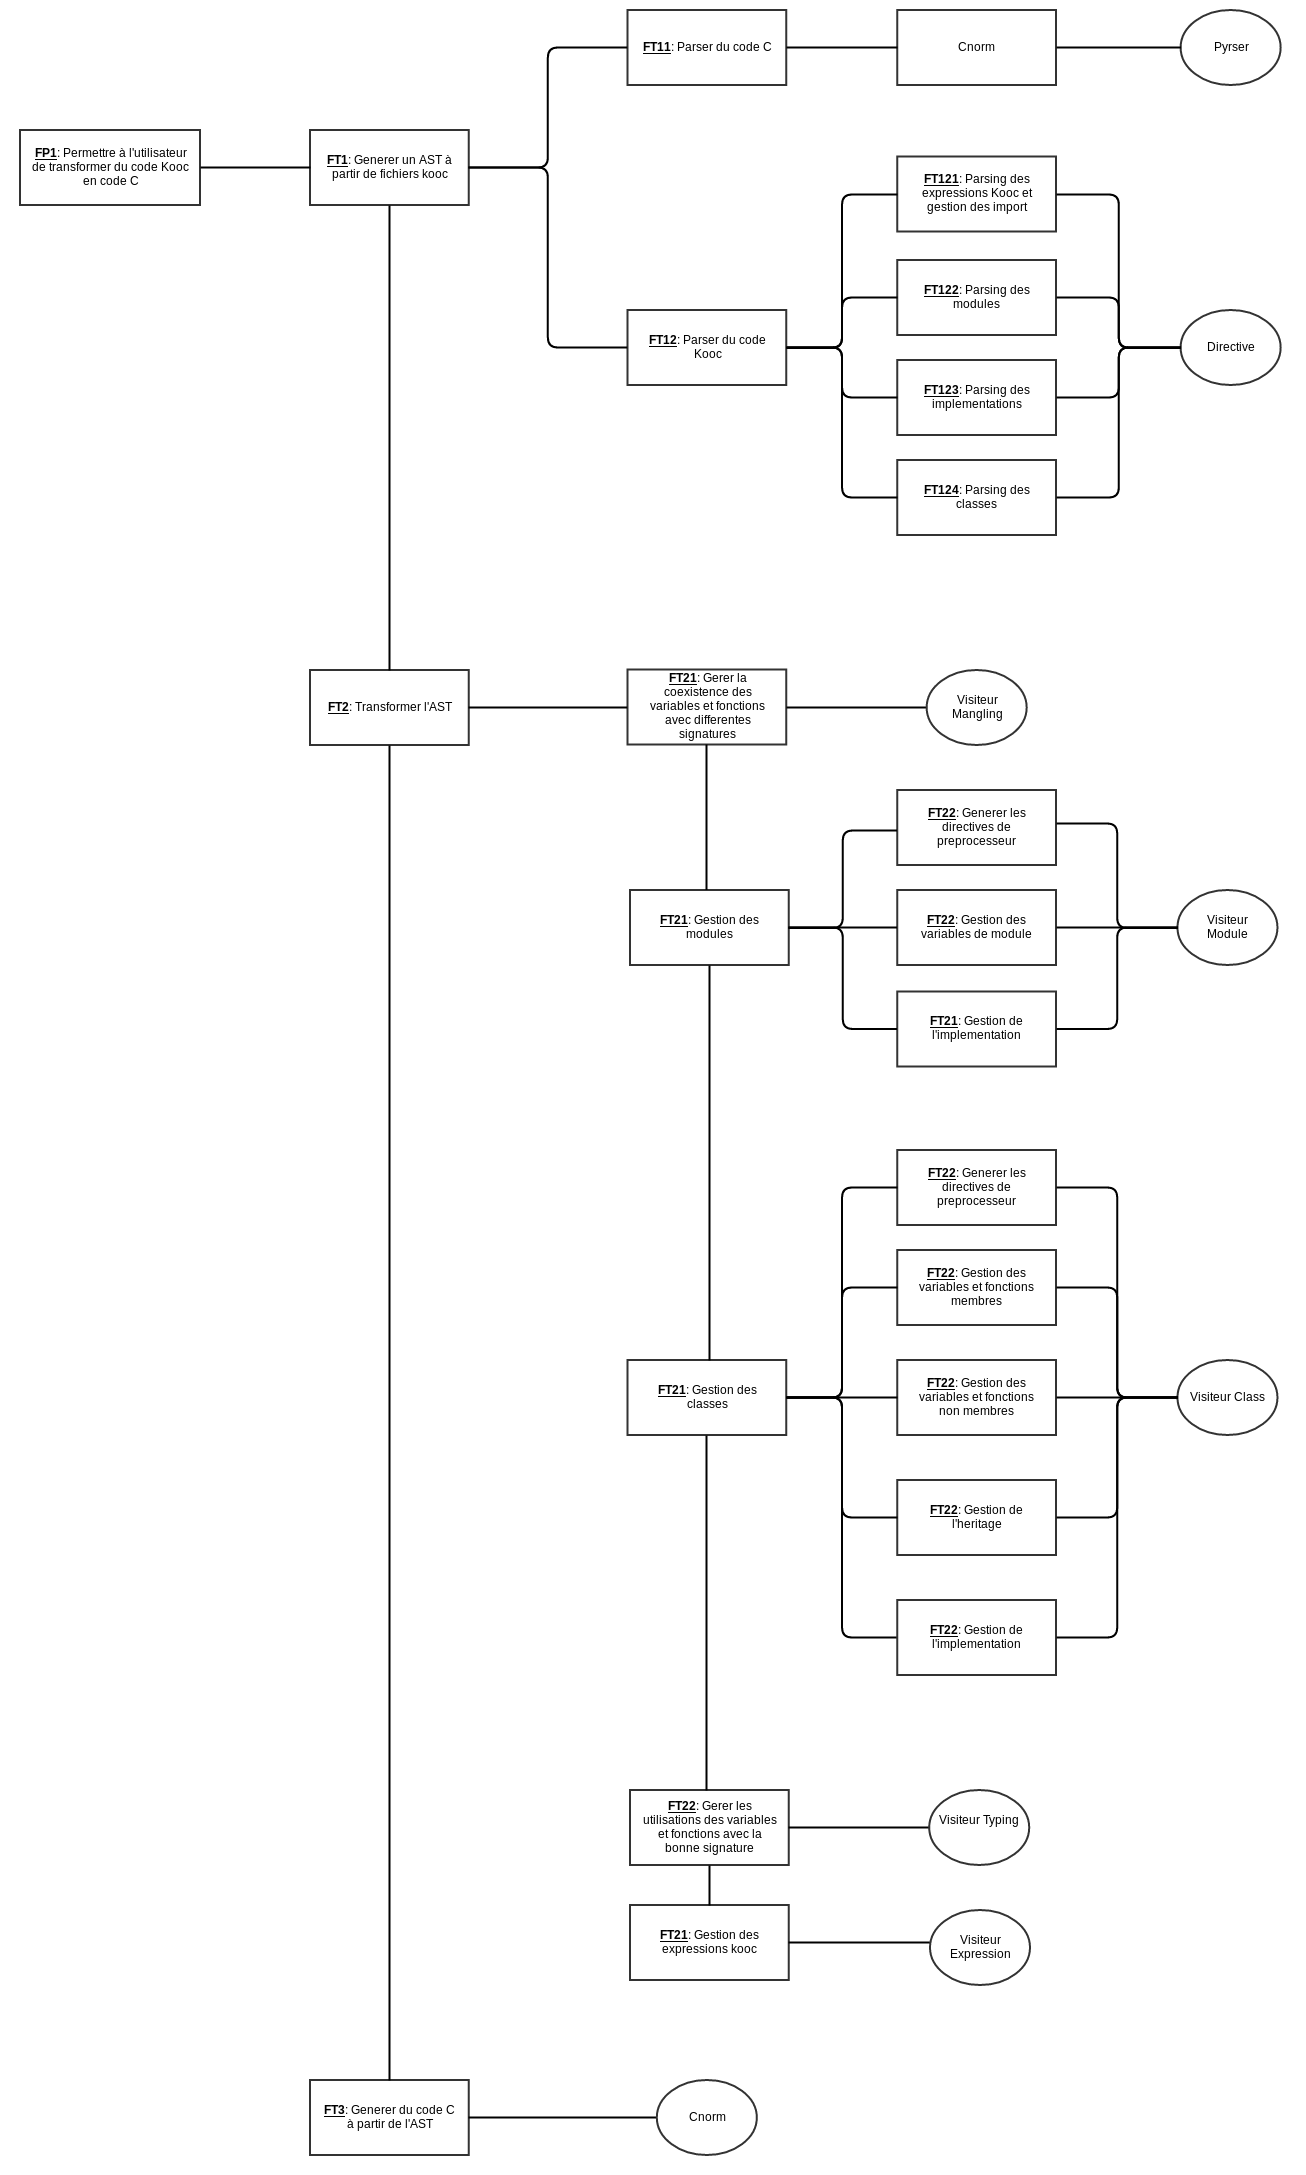
\includegraphics[scale=0.3]{fast.png}
\subsection{Module}
\begin{lstlisting}[title={Module.kh}]
@module         Test
{
  /* Variables relatif au module avec polymorphisme */
  int           a;
  char          a = 'a';
  float         a = 42.0;
  double        a;

  static char   b = 'b';
  static float  b = 21.0;

  /* Fonctions relatif au module avec polymorphisme ad hoc */
  int           f(int foo, float bar);
  float         f(int foo, float bar);
  void          f(const int *foo, const float *bar);
  float         f(int foo);
  float         f(float bar);
  int           f(float bar);
  int           f(int foo);
  void          f(int *foo);
  void          f(float *bar);
}
\end{lstlisting}
\begin{lstlisting}[title={Module.kc}]
/* Gestion des import multiples */
@import "Test.kh"
@import "Test.kh" /* Gestion des commentaires en C */
@import "Test.kh" // Gestion des commentaires C++

@implementation Test
{
  int   f(int foo, float bar)
  {
    return foo+((int)bar);
  }

  float f(int foo, float bar)
  {
    return ((float)foo)+bar;
  }

  void  f(const int *foo, const float *bar)
  {
    printf("int: %i && float: %f\n", *foo, *bar);
  }

  float f(int foo)
  {
    return (float)foo;
  }

  float f(float bar)
  {
    return bar;
  }

  int   f(float bar)
  {
    return (int)bar;
  }

  int   f(int foo)
  {
    return foo;
  }

  void  f(int *foo)
  {
    *foo = [Test.b];            /* Cast implicite */
  }

	f(float *bar)
  {
    *bar = [Test.b];
  }
}
\end{lstlisting}
\subsection{Class}
\begin{lstlisting}[title={Class.kh}]
class  Test
{
  /* Member attributes */
  @member
    {
      int               value = 42;
      float             value = 42.0;
    }
  @member int           secret = 42;

  /* Member functions with the 3 differents syntax */
  @member
    {
      int               get_value();
      float             get_value();
    }
  @member void          set_value(int value);
  @member void          set_value(float value);
  void                  get_class_name(Test *);
  void                  generate_new_secret(Test *);

  /* Some member functions for coplien form */
  @member void          init(int value_int, float value_float);
  void                  init(Test *, float value_float, int value_int);

  /* ! Polymorphism works also with member ! */

  /* Class attributes */
  static int            value = 42;
  static float          value = 42.0;
  int                   secret = 42;

  /* Class functions */
  int                   get_value();
  float                 get_value();
  void                  set_value(int value);
  void                  set_value(float value);
  void                  get_class_name();
  static void           generate_new_secret();
}
\end{lstlisting}
\begin{lstlisting}[title={Class.kc}]
@import "Test.kh"

@implementation Test
{
  @member
    {
      int       get_value()
      {
        return [self.value];
      }

      float     get_value()
      {
        return [self.value];
      }
    }

  @member void  set_value(int number)
  {
    [self.value] = number;
  }

  @member void  set_value(float number)
  {
    [self.value] = number;
  }

  void          get_class_name(Test *this)
  {
    [this generate_new_secret];
    return "Test";
  }

  void          generate_new_secret(Test *that)
  {
    [that.secret] *= 2;
  }

  @member void  init(int value_int, float value_float)
  {
    [self.value] = value_int;
    [self.value] = value_float;
  }

  void          init(Test *self, float value_float, int value_int)
  {
    [self.value] = value_float;
    [self.value] = value_int;
  }

  int           get_value()
  {
    return [Test.value];
  }

  float         get_value()
  {
    return [Test.value];
  }

  void          set_value(int value)
  {
    [Test.value] = value;
  }

  void          set_value(float value)
  {
    [Test.value] = value;
  }

  void          get_class_name()
  {
    [Test generate_new_secret];
    return "Test";
  }

  void          generate_new_secret()
  {
    [Test.secret] *= 2;
  }

}
\end{lstlisting}
\subsection{Heritage}
\begin{lstlisting}[title={Heritage.kh}]
/*
** Les peaux vertes sont des creatures belliqueuses.
** Les orques sont primitifs et pratiquent le chamanisme.
** Les gobelins sont plus intelligents, disciplines et
** pratiquent la magie de bataille.
*/

@class PeauxVertes
{
	        @member
	{
          int   pv;
	  int   attaque;
	  int   agilite;
	}

	@member void    init();

	@virtual void   clean();

	@virtual void   attaque();
        @virtual void   magie();
}

@class Orque : PeauxVertes
{
 	@member void    init();

	@virtual void   clean();

	@virtual void   attaque();
	@virtual void   magie();
}

@class Gobelin : PeauxVertes
{
	@member
	{
          int   parchemins; //necessaire pour jeter une boule de feu
	}

	@member void    init();
	@virtual void   clean();

        @virtual void   magie();
}  
\end{lstlisting}
\begin{lstlisting}[title={Heritage.kc}]
#include <stdio.h>

@implementation PeauxVertes
{
        @member void init()
        {
          this->pv = 0;
          this->attaque = 0;
          this->agilite = 0;
        }

        @virtual void   clean() {}

        @virtual void   attaque()
        {
          puts("Le peau-verte attaque !");
        }

        @virtual void   magie()
        {
          puts("Le peau-verte lance un sort !");
        }
}

@implementation Orque : PeauxVertes
{
        @member void init()
        {
          this->pv = 16;
          this->attaque = 15;
          this->agilite = 8;
        }

        @virtual void   clean() {}

        @virtual void   attaque()
        {
          puts("L'orque attaque avec une massue !");
        }

        @virtual void   magie()
        {
          puts("L'orque fait un rituel chamanique !");
        }

}

@implementation Gobelin : PeauxVertes
{
        @member void init()
        {
          this->pv = 10;
          this->attaque = 9;
          this->agilite = 18;
          this->parchemins = 3;
        }

        @virtual void   clean() {}

        @virtual void   magie()
        {
          if (this->parchemins > 0)
            {
              puts("Le gobelin jette une boule de feu !");
              this->parchemins -= 1;
            }
          else
            puts("Plus de parchemins !");
        }
}
\end{lstlisting}
\subsection{Test inferences}
\begin{lstlisting}[title={testInference.kh}]
@module Test
{
  int   a = 42;
  float a = 42.0;

  void  f();
  void  f(int foo);
  void  f(float bar);
  void  f(int foo, float bar);
  void  f(float bar, int foo);

  int   f();
  int   f(int foo);
  int   f(float bar);
  int   f(int foo, float bar);
  int   f(float bar, int foo);

  float f();
  float f(int foo);
  float f(float bar);
  float f(int foo, float bar);
  float f(float bar, int foo);
}  
\end{lstlisting}
\begin{lstlisting}[title={testInference.kc}]
@import "testInference.kh"

int	main()
{
  int	res_int;
  float	res_float;

  [Test f];				/* void f() */
  [Test f :42];				/* void f(int foo) */
  [Test f :42.0];			/* void f(float bar) */
  [Test f :42 :[Test.a]];		/* void f(int foo, float bar) */
  [Test f :42.0 :[Test.a]];		/* void f(float bar, int foo) */

  res_int = [Test f];			/* int f() */
  res_int = [Test f :42];		/* int f(int foo) */
  res_int = [Test f :42.0];		/* int f(float bar) */
  res_int = [Test f :42 :[Test.a]];	/* int f(int foo, float bar) */
  res_int = [Test f :42.0 :[Test.a]];	/* int f(float bar, int foo) */

  res_float = [Test f];			/* float f() */
  res_float = [Test f :42];		/* float f(float foo) */
  res_float = [Test f :42.0];		/* float f(float bar) */
  res_float = [Test f :42 :[Test.a]];	/* float f(float foo, float bar) */
  res_float = [Test f :42.0 :[Test.a]];	/* float f(float bar, float foo) */

  return 0;
}
\end{lstlisting}
\end{NoHyper}
\end{document}
\grid
